\documentclass[a4paper]{article}
\usepackage[T1]{fontenc}
\usepackage[utf8]{inputenc}
\usepackage{lmodern}
\usepackage{amsmath,amssymb}
\usepackage[top=3cm,bottom=2cm,left=2cm,right=2cm]{geometry}
\usepackage{fancyhdr}
\usepackage{esvect}
\usepackage{xcolor}
\usepackage{tikz}\usetikzlibrary{calc}

\parskip 1em\parindent 0pt

\begin{document}

\pagestyle{fancy}
\fancyhf{}
\setlength{\headheight}{15pt}
\fancyhead[L]{Optique}\fancyhead[R]{Question 13}

% Énoncé
\begin{center}
	\large{\boldmath{\textbf{Différence de marche pour un Michelson monté en coin d’air}}}
\end{center}

% Correction

\begin{center}
    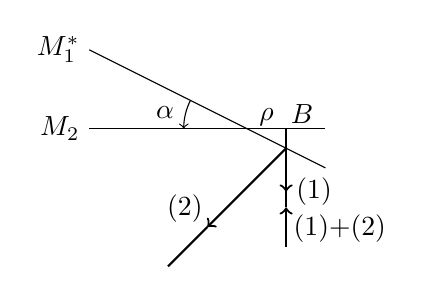
\begin{tikzpicture}
        \draw (-2,0) node[left]{$M_2$} -- (1,0);
        \draw (-2,1) node[left]{$M_1^*$} -- (1,-.5);
        \draw[<-] (-.8,0) node[above left]{$\alpha$} arc (180:153:.8) ;
        \draw[thick,->] (.5,-1.5) -- ++(0,.5) node[below right=-1pt]{(1)+(2)};
        \draw[thick] (.5,-1) -- ++(0,.3);
        \draw[thick,<-] (.5,-.8) node[right]{(1)} -- (.5,0) node[above right=-2pt]{$B$};
        \draw[thick,->] (.5,-.25) -- ++(-1,-1) node[above left=-2pt]{(2)};
        \draw[thick] (-.5, -1.25) -- (-1,-1.75);
        \node at (.25,.15) {$\rho$};
    \end{tikzpicture}
\end{center}
\par

On incline très légèrement le miroir donc \( \alpha \ll 1 \).\\
\fcolorbox{red}{white}{Ainsi \( \delta = 2 \rho \alpha \)}

\end{document}
